\documentclass[12pt,a4paper]{article}
\usepackage[utf8]{inputenc}
\usepackage[english]{babel}
\usepackage{enumerate}
\usepackage{amsmath}
\usepackage{amsfonts}
\usepackage{amssymb}
\usepackage{graphicx}
\usepackage{fourier}
\usepackage[left=2cm,right=2cm,top=2cm,bottom=2cm]{geometry}
\usepackage{commath}
\usepackage{cancel}
\usepackage{placeins}
\author{Juan Carlos Apitz, ID 012523821}
\title{STAT572 - Homework Assignment 7}
\begin{document}

\maketitle

\section*{Exercise 9.19}
\textbf{Kernel Random Sample Generation Using Finite Mixture Method}
\begin{figure}[ht!] 
\begin{center}
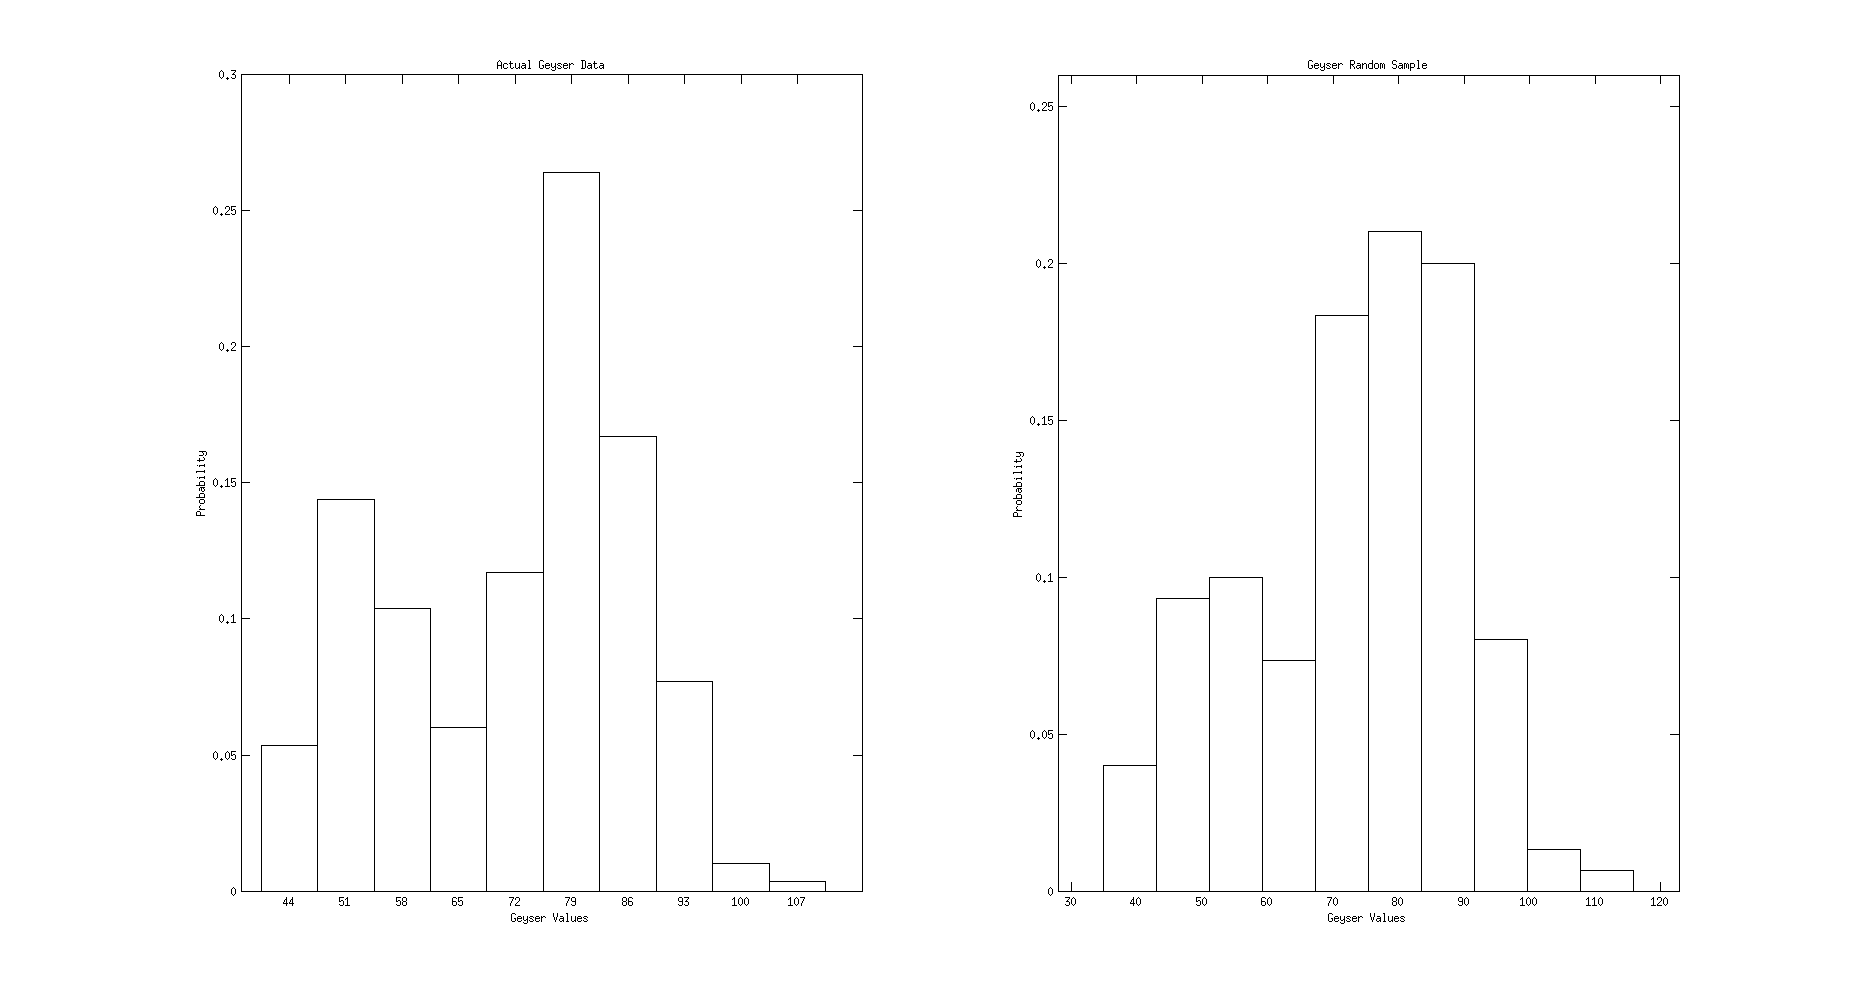
\includegraphics[scale=.35]{q9p19_graph1.png}
\caption{Actual Geyser data (left panel) vs. random sample of size $k=300$ generated from $\hat{f}(x)_{ker}$, the kernel density estimator of the Geyser density (right panel). The random sample generated resembles the Geyser data fairly close. The idea behind using the finite mixture method based on a kernel density estimate is that we use each kernel generated as a "component distribution", where $c=n$ with $n$ being the number of data points used to estimate the density. That means that the weights for the finite mixture process are all equal and calculated as $\frac{1}{n}$. In this example $n=299$, the number of data points in the Geyser dataset.}
\label{q19 fig1}
\end{center}
\end{figure}
\FloatBarrier
\textbf{Code}
\begin{verbatim}
addpath ~/Documents/Stat572/CompStatsToolboxV2;
load geyser
data = geyser; n = length(data);

% choose an appropriate domain
x = linspace(40,110,1000); % domain

% NORMAL KERNEL

% choose smoothing parameter
h = 1.06*std(data)*n^(-1/5);

% initialize vector for estimated pdf
fhat = zeros(size(x));

% evaluate using the normal kernel for each data point
% at all x in the domain
for i=1:n
    % get each kernel function evaluated at x
    % centered at data and weighted by h
    f=exp(-(1/(2*h^2))*(x-data(i)).^2)/sqrt(2*pi)/h;
    % add each ith average f vector to get estimate pdf height
    fhat = fhat+f/n;
end

% Now generate some random variables from this model.
% The model is defined as a kernel density estimation model with n
% component distributions

% The weights for each component kernel is 1/n
% thus create a vector (p1, p1+p2, p1+p2+p3...)
p = (1/n):(1/n):1;

% Set up the random sample generation procedure
k = 300; mus = zeros(1,k);

% this loop generates the means from the kernel vector from the original
% data
for i = 1:k
    u = rand;
    for j = 1:length(p)-1
        if u >= p(j) && u <= p(j+1)
            mus(i) = data(j);
        end
    end
end

% This generates the actual random sample variables
rs = randn(1,k)*h + mus;

% Plots
% Create histograms 
subplot(121);
histdata = hist(data)./n;
xhist = linspace(min(data)+1,max(data)-1,length(histdata));
bar(xhist,histdata,1,'w')
axis([38 115 0 .3]); 
xlabel('Geyser Values'); ylabel('Probability')
title('Actual Geyser Data','FontSize',14)

subplot(122);
histdata = hist(rs)./k;
xhist = linspace(min(rs)+1,max(rs)-1,length(histdata));
bar(xhist,histdata,1,'w')
axis([(min(rs)-10) (max(rs)+10) 0 (max(histdata)+.05)])
xlabel('Geyser Values'); ylabel('Probability')
title('Geyser Random Sample','FontSize',24)
\end{verbatim}
\clearpage

\section*{In-class Assignment - Kernel vs Finite Mixture Random Sampling}
\textbf{Part a)}\\
\textbf{Create Density Estimates from Kernel, Finite Mixture, and Histogram}\\

\begin{figure}[ht!] 
\begin{center}
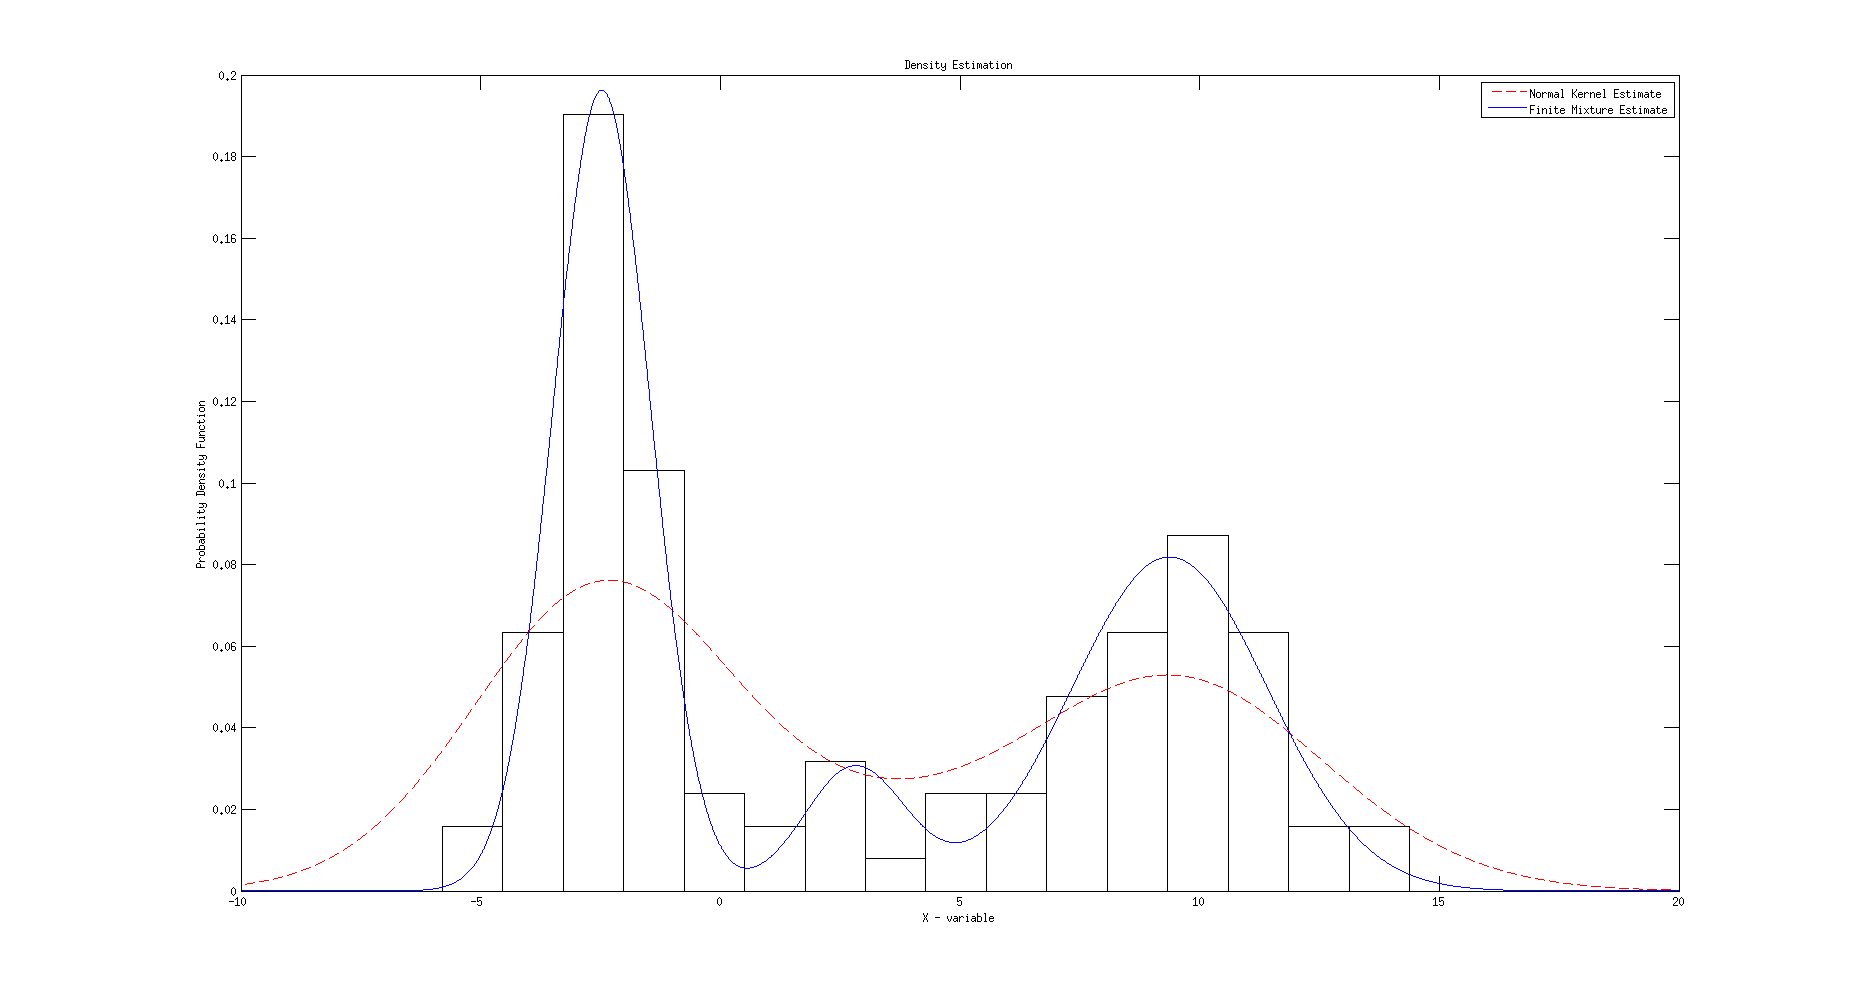
\includegraphics[scale=.2]{inclass7p1_graph1}
\caption{In this implementation of density estimation using the kernel method the smoothing constant is chosen to be $h=1.06\hat{\sigma}n^{\frac{1}{5}}$ based on Silverma's rule. As we can see, the kernel density estimate appears much more smoother that that of the finite mixture. This is expected because the model chosen for the finite mixture closely resembles the actual data, so one would expect that the finite mixture estimate would closely resemble the data. But what if the model chosen does not include all the actual components in the mixture?. In the next graph we choose a different smoothing parameter for the kernel estimate.}
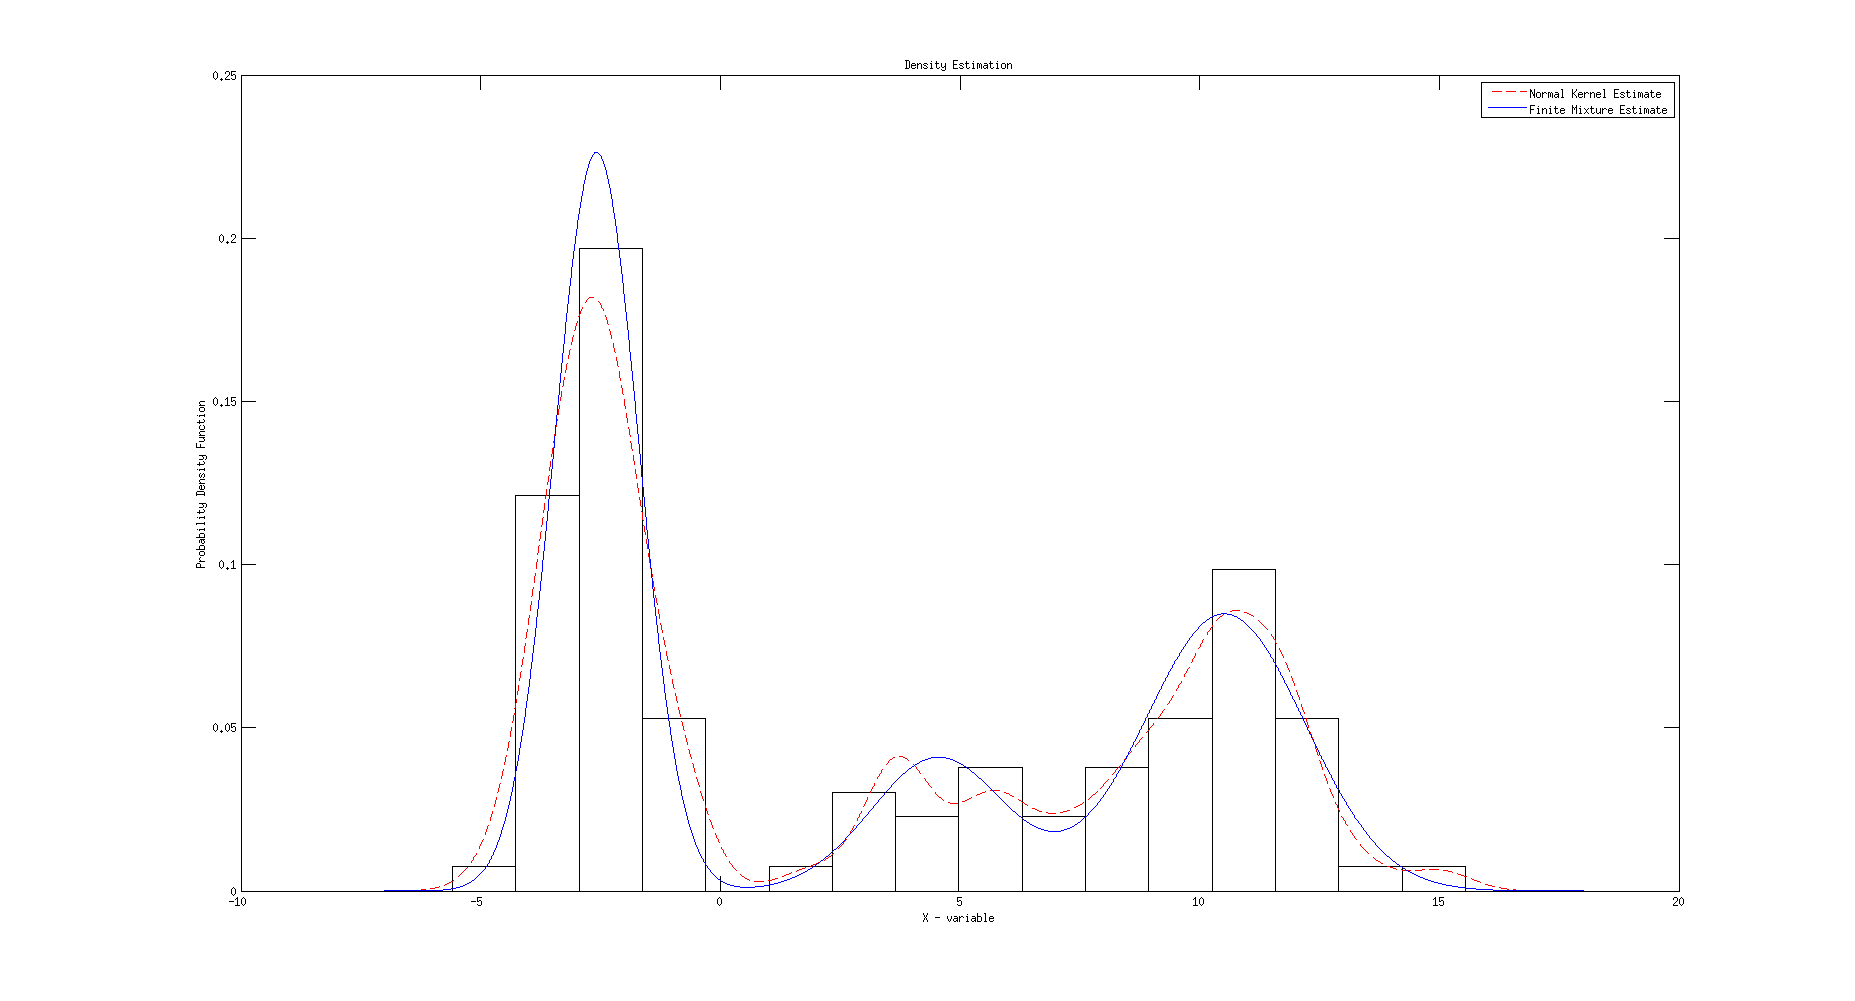
\includegraphics[scale=.2]{inclass7p1_graph2}
\caption{In this density estimation implementation we increase the roughness of the kernel estimate by choosing a new $h^{*}=\frac{h}{4}$. Now we see that by increasing roughness we actually get a closer match between the finite mixture and the kernel density estimate. This example emphasizes the importance of our choice of $h$ when estimating densities.}
\label{inclass fig1}
\end{center}
\end{figure}
\FloatBarrier
\textbf{Code}
\begin{verbatim}
addpath ~/Documents/Stat572/CompStatsToolboxV2
% 1. CREATE 3-TERM DATASET, n=100
data = [normrnd(-2.5,1,1,50),normrnd(4.5,sqrt(2),1,15)...
    ,normrnd(10.5,sqrt(3),1,35)];
n = length(data);

% 2. ESTIMATE THE DENSITY FOR ABOVE DATA USING NORMAL KERNEL
% choose an appropriate domain
x = linspace(-10,20,5000); % domain

% choose smoothing parameter
h = 1.06*std(data)*n^(-1/5); 

% evaluate using the normal kernel for each data point 
% at all x in the domain
fhat = zeros(size(x));
for i=1:n
    % get each kernel function evaluated at x
    % centered at data and weighted by h
    f=exp(-(1/(2*h^2))*(x-data(i)).^2)/sqrt(2*pi)/h;
    % add each ith average f vector to get estimate pdf height
    fhat = fhat+f/(n);
end

% 3. USE FINITE MIXTURE TO ESTIMATE DENSITY OF DATA, c=3
% Set initial model to means at 50 and 80.
muin = [-1, 4, 9];
% Set mixing coefficients equal.
piesin = [0.5, 0.25, 0.25];
% Set initial variances to 1.
varin = [1, 1, 1];
max_it = 100;
tol = 0.001;
% Call the finite mixtures.
[pies,mus,vars]=...
    csfinmix(data,muin,varin,piesin,max_it,tol);

% 4. PLOT THE RESULTS

% Histogram estimate of the PDF
% Use Normal Reference Rule for bin width
% of frequency histogram.
h = 2.15*sqrt(var(data))*n^(-1/5)*0.25;
t0 = min(data)-1;
tm = max(data)+1;
bins = t0:h:tm;
vk = histc(data,bins);
vk(end) = [];
fhath = vk/(n*h);
bc = (t0+h/2):h:(tm-h/2);

% Plotting
bar(bc,fhath,1,'w')
hold on
xlabel('X - variable')
ylabel('Probability Density Function')
title('Density Estimation')
linenorm = plot(x,fhat,'--r');
hold on
linemix = csplotuni(pies,mus,vars,min(x),max(x),length(x));
legend([linenorm,linemix],'Normal Kernel Estimate','Finite Mixture Estimate')
hold off
\end{verbatim}
\clearpage
\textbf{Part b)}\\
\textbf{Generate Random Samples from Kernel Method and from Finite Mixture and Compare}\\
\begin{figure}[ht!] 
\begin{center}
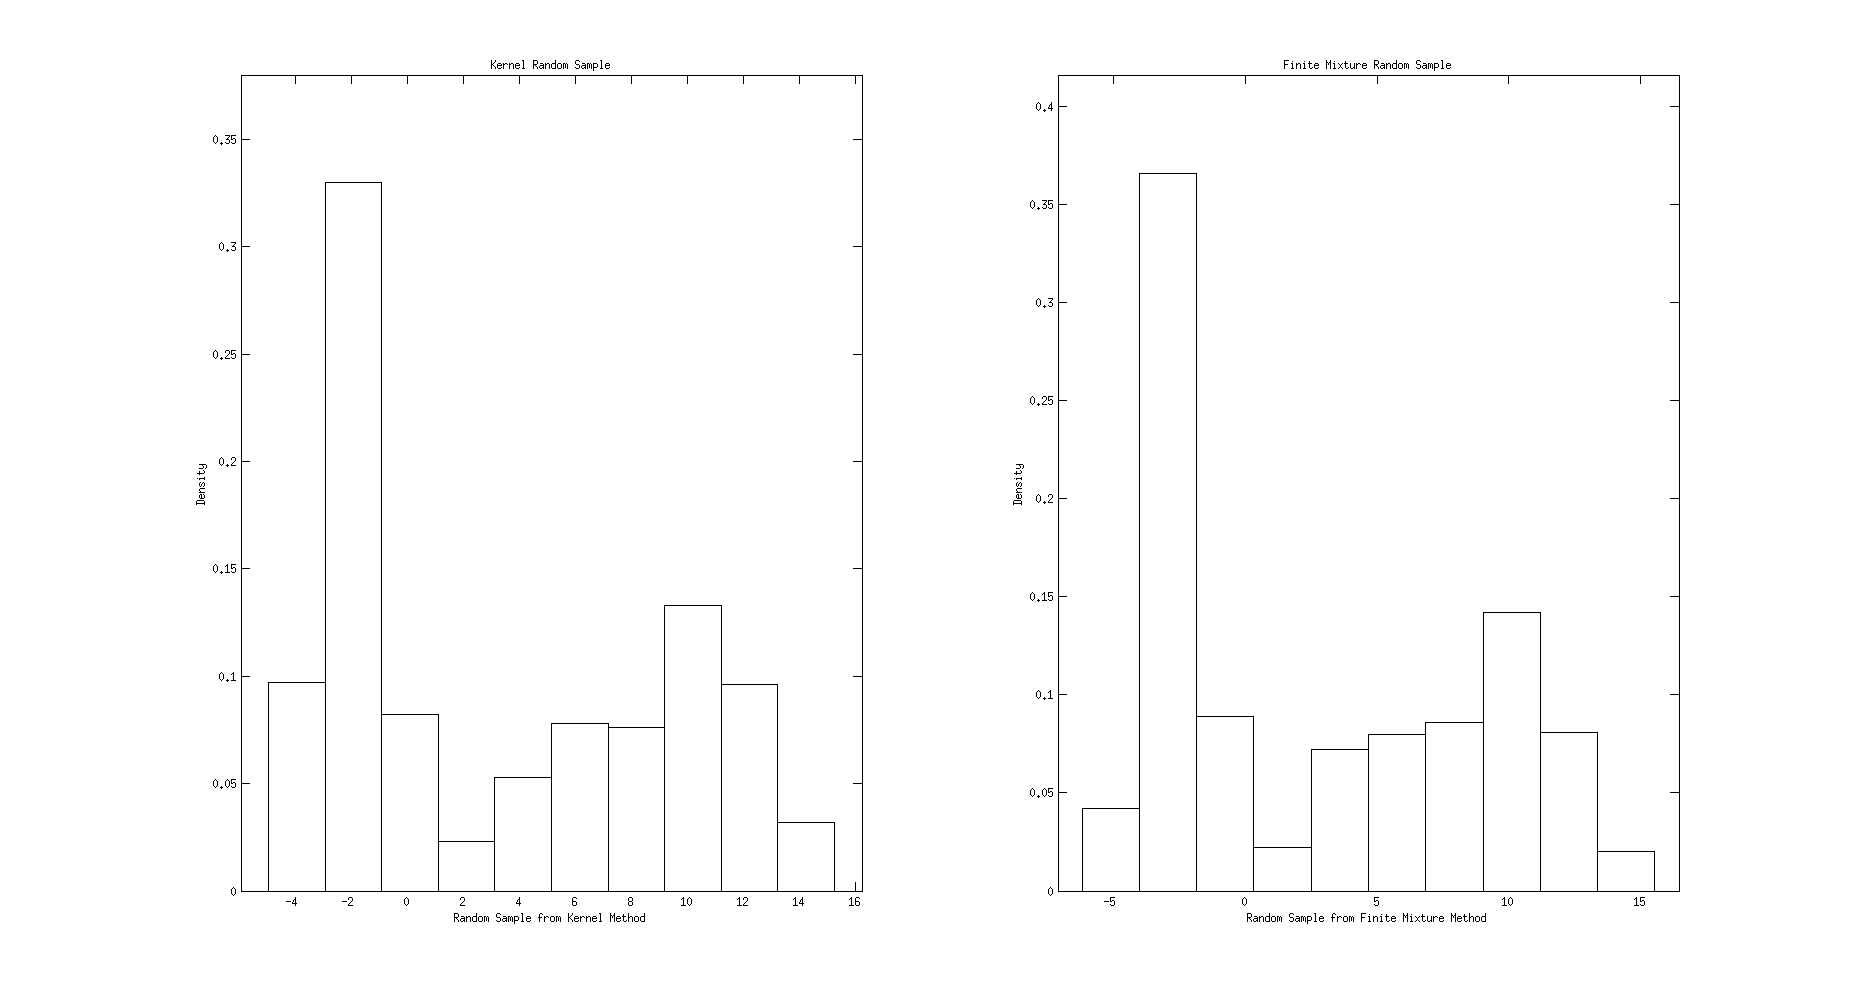
\includegraphics[scale=.35]{inclass7p1_graph3}
\caption{The left panel is the histogram of the random sample generated using the kernel based finite mixture random sampling algorithm. On the right is the random sample generated by the finite mixture estimate using an initial 3-component model with means: $\hat{\mu_1}=-1$, $\hat{\mu_2}=4$,  $\hat{\mu_3}=9$, variances: $\hat{\sigma}_1^2=\hat{\sigma}_2^2=\hat{\sigma}_3^2=1$, and weights: $\hat{p_1}=0.5$, $\hat{p_2}=0.25$,  $\hat{p_3}=0.25$. The random samples seem fairly consistent, which indicates that both approaches are valid and consistent.
}
\label{inclass fig2}
\end{center}
\end{figure}
\FloatBarrier
\textbf{Code}
\begin{verbatim}
% GENERATE RANDOM SAMPLES OF SIZE 1000 FROM EACH METHOD

% Kernel Method
% The model is defined as a kernel density estimation model with n
% component distributions

% The weights for each component kernel is 1/n
% thus create a vector (p1, p1+p2, p1+p2+p3...)
p = (1/n):(1/n):1;

% Set up the random sample generation procedure
k = 1000; musk = zeros(1,k);

% this loop generates the means from the kernel vector from the original
% data
for i = 1:k
    u = rand;
    for j = 1:length(p)-1
        if u >= p(j) && u <= p(j+1)
            musk(i) = data(j);
        end
    end
end

% This generates the actual random sample variables
rsk = rand(1,k)*h + musk;

% Finite mixture method

% Now generate some random variables from this model.
% Get the true model to generate data from this.
rsmx = zeros(k,1);
% Now generate k random variables. First find
% the number that fall in each one.
r = rand(1,k);
% Find the number generated from component 1.
ind1 = length(find(r <= pies(1)));
ind2 = length(find(r > pies(1) & r <= pies(1)+pies(2)));
% Create some mixture data. Note that the 
% component densities are normals.
rsmx(1:ind1) = randn(ind1,1)*sqrt(vars(1)) + mus(1);
rsmx(ind1+1:ind1+ind2) = randn(ind2,1)*sqrt(vars(2)) + mus(2);
rsmx(ind1+ind2+1:k) = randn(k-ind1-ind2,1)*sqrt(vars(3)) + mus(3);

% 6. DRAW HISTOGRAM OF BOTH RANDOM SAMPLES AND COMPARE

% Create histograms 
figure (2)
subplot(121);
histdata = hist(rsk)./k;
xhist = linspace(min(rsk)+1,max(rsk)-1,length(histdata));
bar(xhist,histdata,1,'w')
axis([(min(rsk)-1) (max(rsk)+1) 0 (max(histdata)+.05)]) 
xlabel('Random Sample from Kernel Method'); ylabel('Density')
title('Kernel Random Sample')

subplot(122);
histdata = hist(rsmx)./k;
xhist = linspace(min(rsmx)+1,max(rsmx)-1,length(histdata));
bar(xhist,histdata,1,'w')
axis([(min(rsmx)-1) (max(rsmx)+1) 0 (max(histdata)+.05)])
xlabel('Random Sample from Finite Mixture Method'); ylabel('Density')
title('Finite Mixture Random Sample')
\end{verbatim}

\end{document}